\documentclass[10pt,a4paper,twocolumn]{article}
\usepackage[utf8]{inputenc}
\usepackage{amsmath}
\usepackage{amsfonts}
\usepackage{amssymb}
\usepackage{graphicx}
\usepackage{subcaption}
\author{Sven Thijssen, Emile Valcke}
\title{Inverse Reinforcement Learning}
\begin{document}
\maketitle

\section{Introduction}
Reinforcement Learning is a learning task in which an agent tries to optimize its actions, based on its state and rewards in a given environment. For Inverse Reinforcement Learning, the agent is not aware of the rewards and tries to learn the reward function by looking at an expert's behaviour. n optimal policy that maximizes the cumulative rewards. IRL accomplishes two tasks: reward learning and apprenticeship learning. Reward learning is about estimating the reward function as accurately as possible. Apprenticeship learning is about observating an expert and using it to decide it's own policy or behaviour. The main goal of this to get an optimal policy that maximizes the cumulative rewards.  

\section{Literature}
Our starting point was \textit{Inverse Reinforcement Learning} by Pieter Abbeel and Andrew Y. Ng in the \textit{Encyclopedia of Machine Learning} \cite{sammut2011encyclopedia}. According to its definition, the goal of inverse reinforcement learning is to extract a reward function, given observed behavior of an agent in an environment. The main motivation for this learning task is the difficulty of defining rewards for actions performed by the agent. In this paper and all the other papers we read about Inverse Reinforcement Learning, the problem environment was modelled by the Markov Decision Process framework. It is a model of a control process where an agent has to take decisions and performs actions to go to new states.\\

A finite Markov Decision Process consists of a tuple (S,A,T,R) where:

\begin{itemize}
\item S is a set of states
\item $A = \{a_1,...,a_k\}$ is a set of k actions
\item T is a probability function T :S x A x S $->$ [0,1]
\item R is a reward function R: S x A $->$ ${\rm I\!R}$\\
\end{itemize}



\section{Creative part}
For the creative part of this assignment, we have opted to implement the algorithm suggested by Pieter Abbeel and Andrew Y. Ng  in the paper \textit{Apprenticeship Learning by Inverse Reinforcement Learning} \cite{abbeel2004apprenticeship}. The incentive to implement an algorithm for inverse reinforcement learning was to fully comprehend the concept. As the saying goes, ``practice makes perfect''. The initial suggestion for the creative part was inverse reinforcement learning applied to Tic-Tac-Toe. However, because of its stochastic environment, this would have led us too far for the assignment. Therefore we have opted to apply inverse reinforcement learning on a grid world such that the concepts can easily be visualized and explained.

\subsection{Implementation}
In the algorithm, multiple approaches are suggested to compute the weights $w$. One such approach would be to use a quadratic programming solver where the problem is defined as follows:

$$\max\limits_{t, w} t$$\\
s.t. $$w^T \mu_E \geq w^T \mu^{(j)} + t, j= 0,...,i-1$$
$$\|w\|_2 \leq 1$$

Another approach is to use a projection method in which the feature expectations of a policy are recalculated in each iteration. From a practical standpoint, this seemed to be the best method to use.

\subsection{Environment}
The environment on which we tested our implementation is the bicycle storage next to the Computer Science building from KU Leuven. Based on an aerial image from Google Maps (Figure \ref{fig:google}), we created a grid world environment (Figure \ref{fig:gridworld}). For each cell, we defined the following binary features:

\begin{table}[h]
\centering
\begin{tabular}{|l|l|l|}
	\hline
	Feature		&	Meaning		&	Representation\\\hline
	$\phi_0$		&	Ground		&	Brown\\
	$\phi_1$		&	Obstacle		&	Grey\\
	$\phi_2$		&	Water		&	Blue\\
	$\phi_3$		&	People		&	x\\
	\hline
\end{tabular}
\caption{Features for the grid world}
\end{table}

The aim is to learn a policy $\pi$, based on an expert demonstration $\zeta$ such that we can recover the rewards for the states in the grid world.

Our initial approach was different however. The idea was to guide the agent towards a goal position (marked by $G$ in Figure \ref{fig:gridworld}) by having a feature which represented the distance from that state to the goal state.
We both tested linearly decreasing distances and exponentially decreasing distances for states which are positioned further from the goal position. This tended not to work well, possibly because of the fact that it is too fine-grained.

\begin{figure}[h]
\begin{subfigure}[b]{0.5\textwidth}
	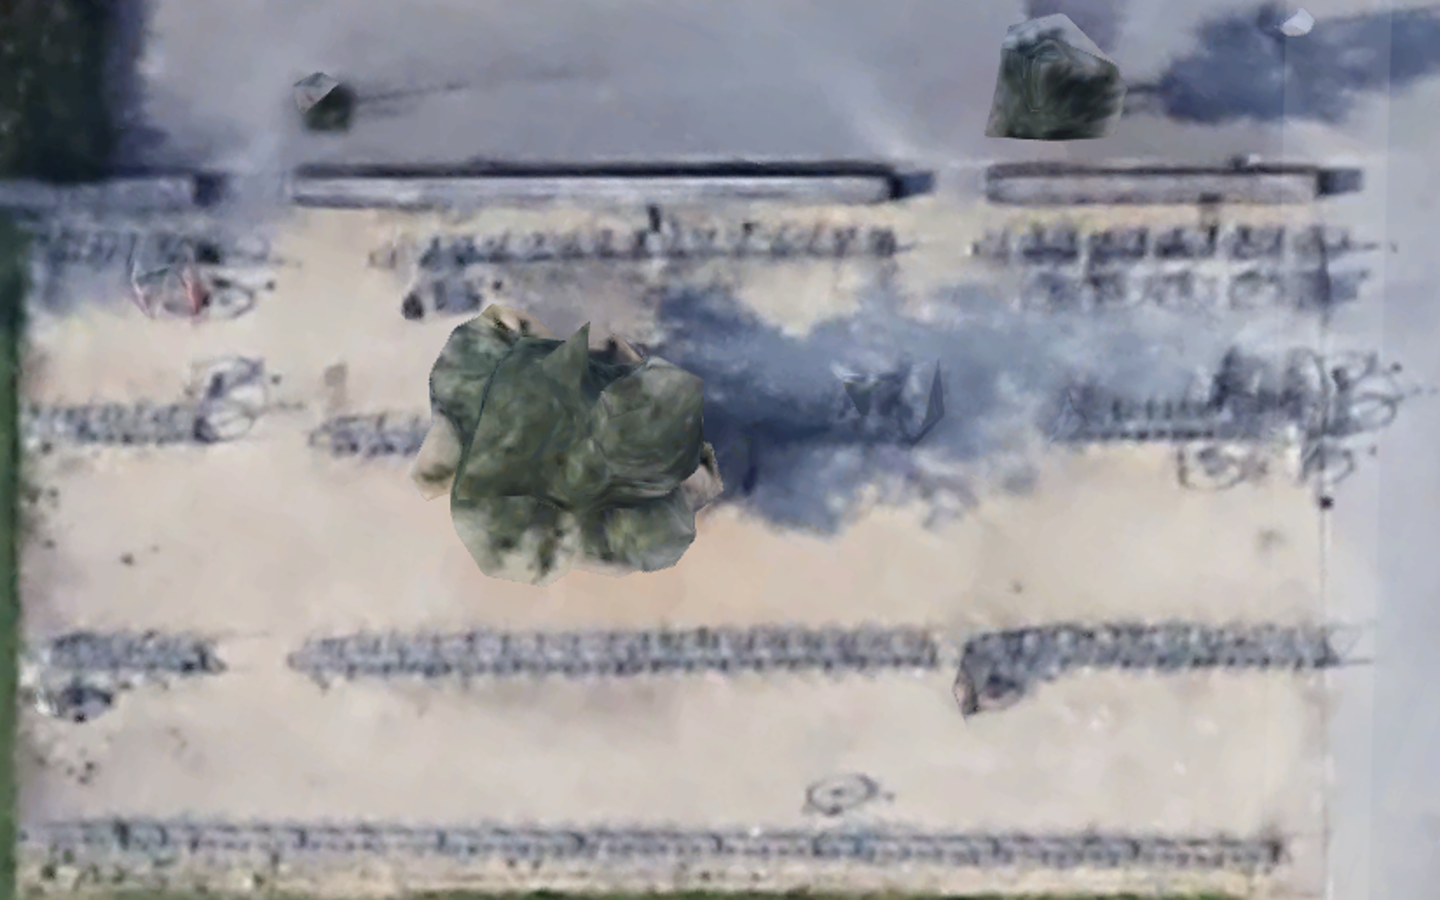
\includegraphics[width=\textwidth]{google}
	\caption{Aerial image of the environment}
	\label{fig:google}
\end{subfigure}
\begin{subfigure}[b]{0.5\textwidth}
	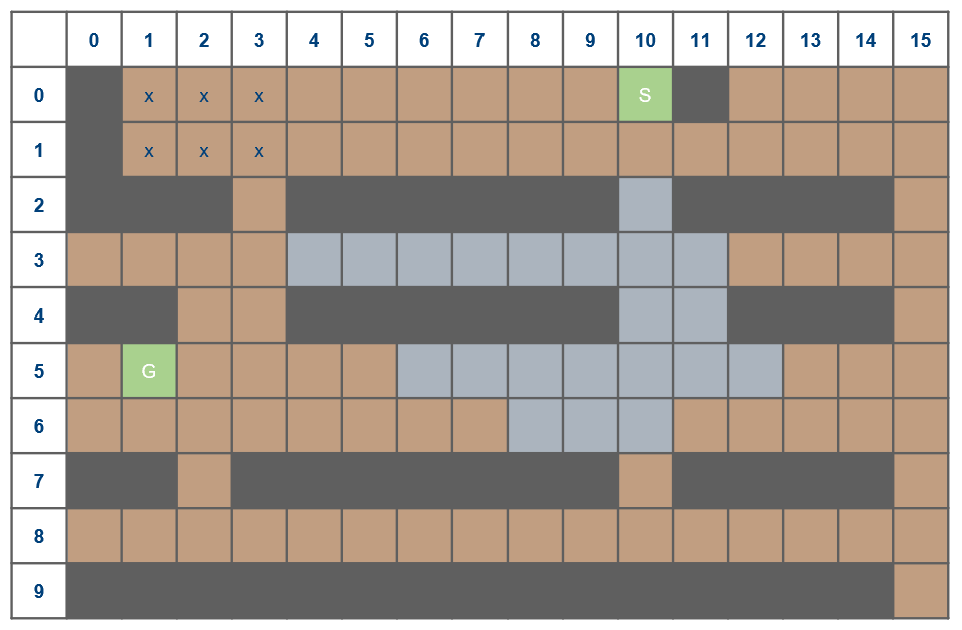
\includegraphics[width=\textwidth]{gridworld}
	\caption{Grid world of the environment}
	\label{fig:gridworld}
\end{subfigure}
\end{figure}

\subsection{Experiments}
To gain insight in the solutions from the algorithm, we made plots of the error $t$ and the weights $w_i$ for the features $\phi_i$.

\begin{figure}[h]
\begin{subfigure}[b]{0.5\textwidth}
	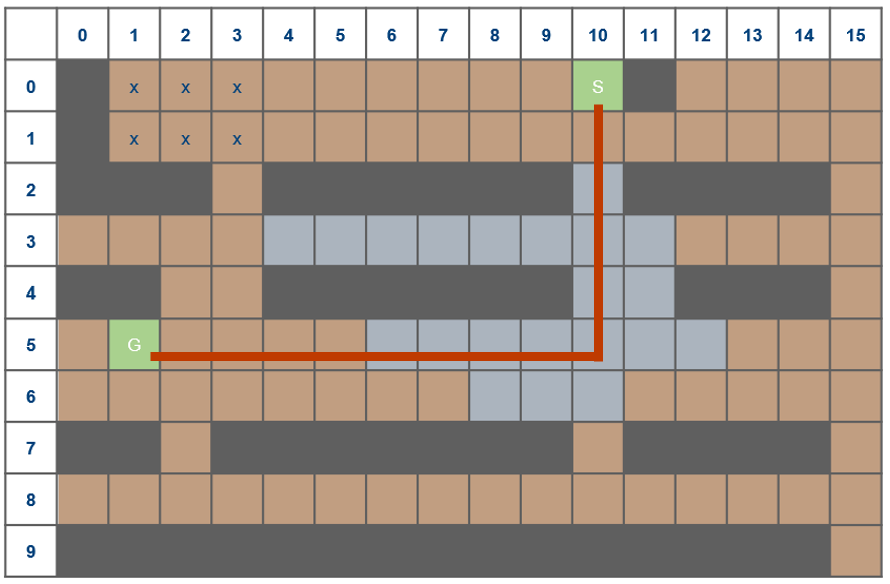
\includegraphics[width=\textwidth]{experiment_1_gridworld}
	\caption{Grid world with expert trajectory}
	\label{fig:experiment1trajectory}
\end{subfigure}
\begin{subfigure}[b]{0.5\textwidth}
	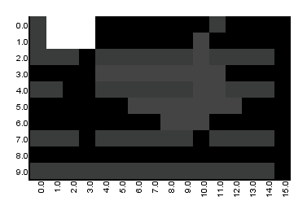
\includegraphics[width=\textwidth]{experiment_1_heatmap}
	\caption{Heat map of the rewards}
	\label{fig:experiment1heatmap}
\end{subfigure}
\end{figure}

As we can observe in Figure \ref{fig:experiment1t}, the error $t$ drops dramatically in the first iterations and then slowly converges to zero. In Figure \ref{fig:experiment1w} we see the respective values for $w$ over time. The values fluctuate around zero. This might be due to the fact that the problem is ill-posed.

\begin{figure}
\begin{subfigure}[b]{0.5\textwidth}
	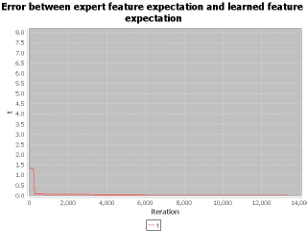
\includegraphics[width=\textwidth]{experiment_1_t}
	\caption{Grid world with expert trajectory}
	\label{fig:experiment1t}
\end{subfigure}
\begin{subfigure}[b]{0.5\textwidth}
	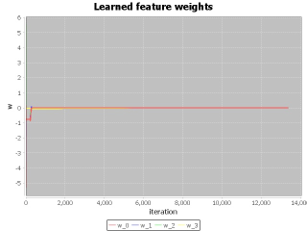
\includegraphics[width=\textwidth]{experiment_1_w}
	\caption{Heat map of the rewards}
	\label{fig:experiment1w}
\end{subfigure}
\end{figure}

For a second expert trajectory, where the agent tends to prefer the features ground and people, we have set the threshold to a bigger value: $0.1$ to avoid the slow convergence. 

\begin{figure}[h]
\begin{subfigure}[b]{0.5\textwidth}
	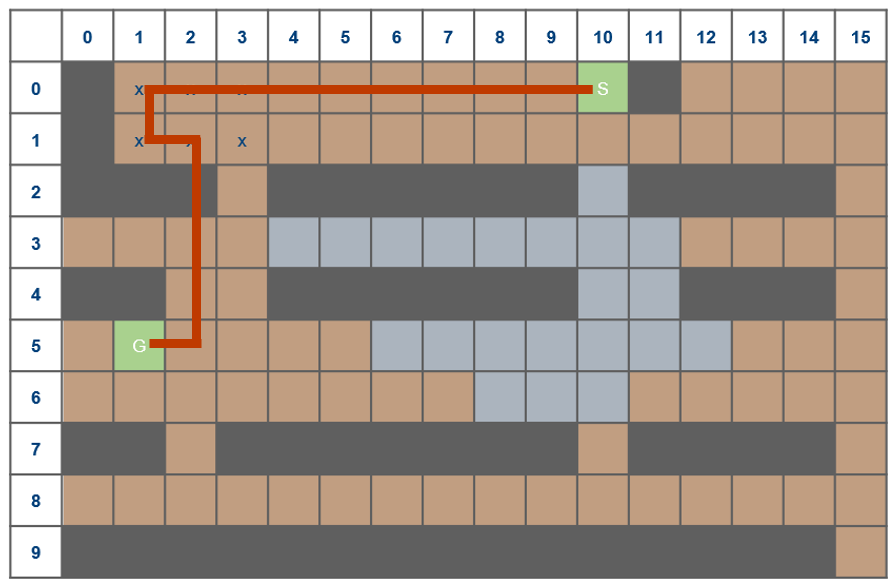
\includegraphics[width=\textwidth]{experiment_2_gridworld}
	\caption{Grid world with expert trajectory}
	\label{fig:experiment1trajectory}
\end{subfigure}
\begin{subfigure}[b]{0.5\textwidth}
	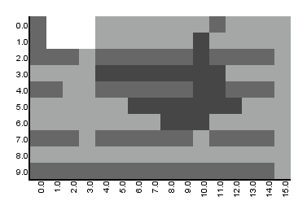
\includegraphics[width=\textwidth]{experiment_2_heatmap}
	\caption{Heat map of the rewards}
	\label{fig:experiment1heatmap}
\end{subfigure}
\end{figure}

\begin{figure}
\begin{subfigure}[b]{0.5\textwidth}
	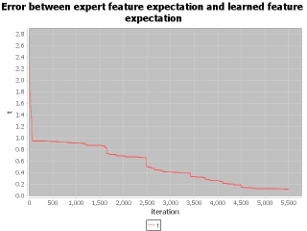
\includegraphics[width=\textwidth]{experiment_2_t}
	\caption{Grid world with expert trajectory}
	\label{fig:experiment1t}
\end{subfigure}
\begin{subfigure}[b]{0.5\textwidth}
	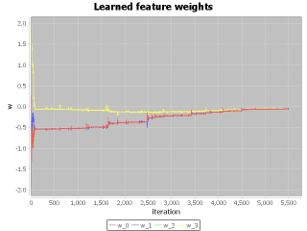
\includegraphics[width=\textwidth]{experiment_2_w}
	\caption{Heat map of the rewards}
	\label{fig:experiment1w}
\end{subfigure}
\end{figure}

%TODO q-learning
%TODO softmax
%TODO loops solution



\subsection{Experiments}

\section{Conclusion}

\bibliography{references} 
\bibliographystyle{ieeetr}



\end{document}